\documentclass{beamer}
\usepackage[utf8]{inputenc}

\usetheme{Madrid}
\usecolortheme{seahorse}

% For Polish langage
\usepackage[T1]{fontenc}
% \usepackage[polish]{babel}

% For strikethrough text
\usepackage{ulem}

% For tables
\usepackage{multirow}
\usepackage{pdflscape}
\usepackage{colortbl}
\usepackage{tabulary}
\usepackage{etoolbox}
\usepackage{makecell}
\newcolumntype{P}[1]{>{\centering\arraybackslash}p{#1}}

% For figures
\usepackage{caption}
\usepackage{subcaption}

% For math
\usepackage{amsmath,amsfonts}

% For inline code listings
\usepackage{listings}
\usepackage{xparse}
\usepackage{xcolor}
\lstdefinestyle{py}{
  language=Python,
  basicstyle=\small\ttfamily,
  commentstyle=\color{green!40!black},
  keywordstyle=\color{blue},
  numberstyle=\tiny\color{gray},
  numbers=left,
  numbersep=5pt,
  backgroundcolor=\color{white},
  showspaces=false,
  showstringspaces=false,
  frame=single,
  rulecolor=\color{black},
  tabsize=4,
  captionpos=b,
  breaklines=true,
  breakatwhitespace=true,
  title=\lstname,
  caption=\lstname
}

% For algorithms
\usepackage{algorithm,algpseudocode}


% Arrows
\usepackage{tikz}
\usetikzlibrary{shapes.arrows}
\tikzset{
    myarrow/.style={
        draw,
        fill=orange,
        single arrow,
        minimum height=5ex,
        single arrow head extend=1ex
    }
}
\newcommand{\arrowup}{\tikz [baseline=-0.5ex]{\node [myarrow,rotate=90] {};}}
\newcommand{\arrowdown}{\tikz [baseline=-1ex]{\node [myarrow,rotate=-90] {};}}

% Title page
\title[WAW 2024]{19th Workshop on Modelling and Mining Networks}
\subtitle{Network Diffusion --- Framework to Simulate Spreading Processes in Complex Networks}
\author[Micha{\l} Czuba et al.]{
    \textbf{Micha{\l} Czuba} \inst{1},
    Mateusz Nurek \inst{1},
    Damian Serwata \inst{1},
    Yu-Xuan Qi \inst{2},
    Mingshan Jia \inst{2},
    Katarzyna Musial \inst{2},
    Rados{\l}aw Michalski \inst{1},
    Piotr Br{\'o}dka \inst{1}
}
\institute[]{
  \inst{1} Wroc{\l}aw University of Science and Technology\\
  \inst{2} University of Technology Sydney
}
\date[05.06.2024]{05.06.2024}
\logo{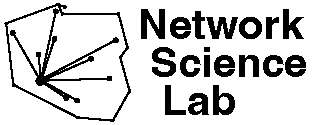
\includegraphics[height=0.5cm]{figures/nsl.pdf}}

\AtEndDocument{
    \addtocounter{framenumber}{-1}
    \begin{frame}[c]
        \centering
        \begin{huge}
            Thank you for your attention!
        \end{huge}
        \begin{figure}
            
\includegraphics[width=5cm]{figures/qr_code2.pdf}
        \end{figure}
        If you like \lstinline[style=py]{network-diffusion} please star the repo :)
    \end{frame}
}

\begin{document}

\frame{\titlepage}

\begin{frame}{Agenda}
    In this talk, I will introduce a computational library --- \lstinline[style=py]{network-diffusion}.
    Here is the agenda:
    \tableofcontents
\end{frame}

\section{Motivation}

\begin{frame}{\secname}
    Spreading phenomena are one of the issues considered by a network science. They can be obeserved
    in various areas like: dynamics of political opinions, marketing campaigns, spread of epidemics,
    computer viruses, etc.
    \begin{figure}
        \centering
        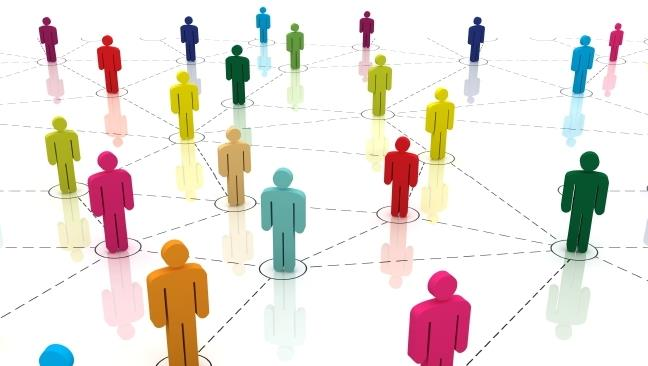
\includegraphics[width=.7\textwidth]{figures/social_network.jpg}
        \caption{Artistic representation of a social network.\footnote{Source: \url{
        www.uniroma3.it/articoli/seminario-biased-opinion-dynamics-when-the-devil-is-in-the-details-138122}
        }}
    \end{figure}
\end{frame}

\begin{frame}{\secname}
    \onslide<1->{Analytical approaches are often insufficient for large graphs, prompting researchers to use 
    computational methods, i.e. simulators.}
    \onslide<2->{\begin{center}
        \vspace{1em}
        \arrowdown
        \vspace{1em}
    \end{center}
    Thus, like in other branches of computer science, there have been developed tools which addres 
    that issue, allowing to avoid starting from scratch and enhancing the reproducibility
    of results.}
\end{frame}

\begin{frame}{\secname}
    \begin{columns}[T]
        \begin{column}{.35\textwidth}
            There is a bunch of tools that helps in sumulating diffusion processes in networks:
            \begin{itemize}
                \item \textbf{NDlib}\cite{ndlib},
                \item GLEaMviz\cite{gleam},
                \item SimInf\cite{siminf},
                \item STEM\cite{stem},
                \item EpiModel\cite{jenness2018epimodel},
                \item Sispread\cite{sispread},
                \item ...
            \end{itemize}
        \end{column}
        \hfill
        \begin{column}{.60\textwidth}
            \begin{figure}[ht]
                \centering
                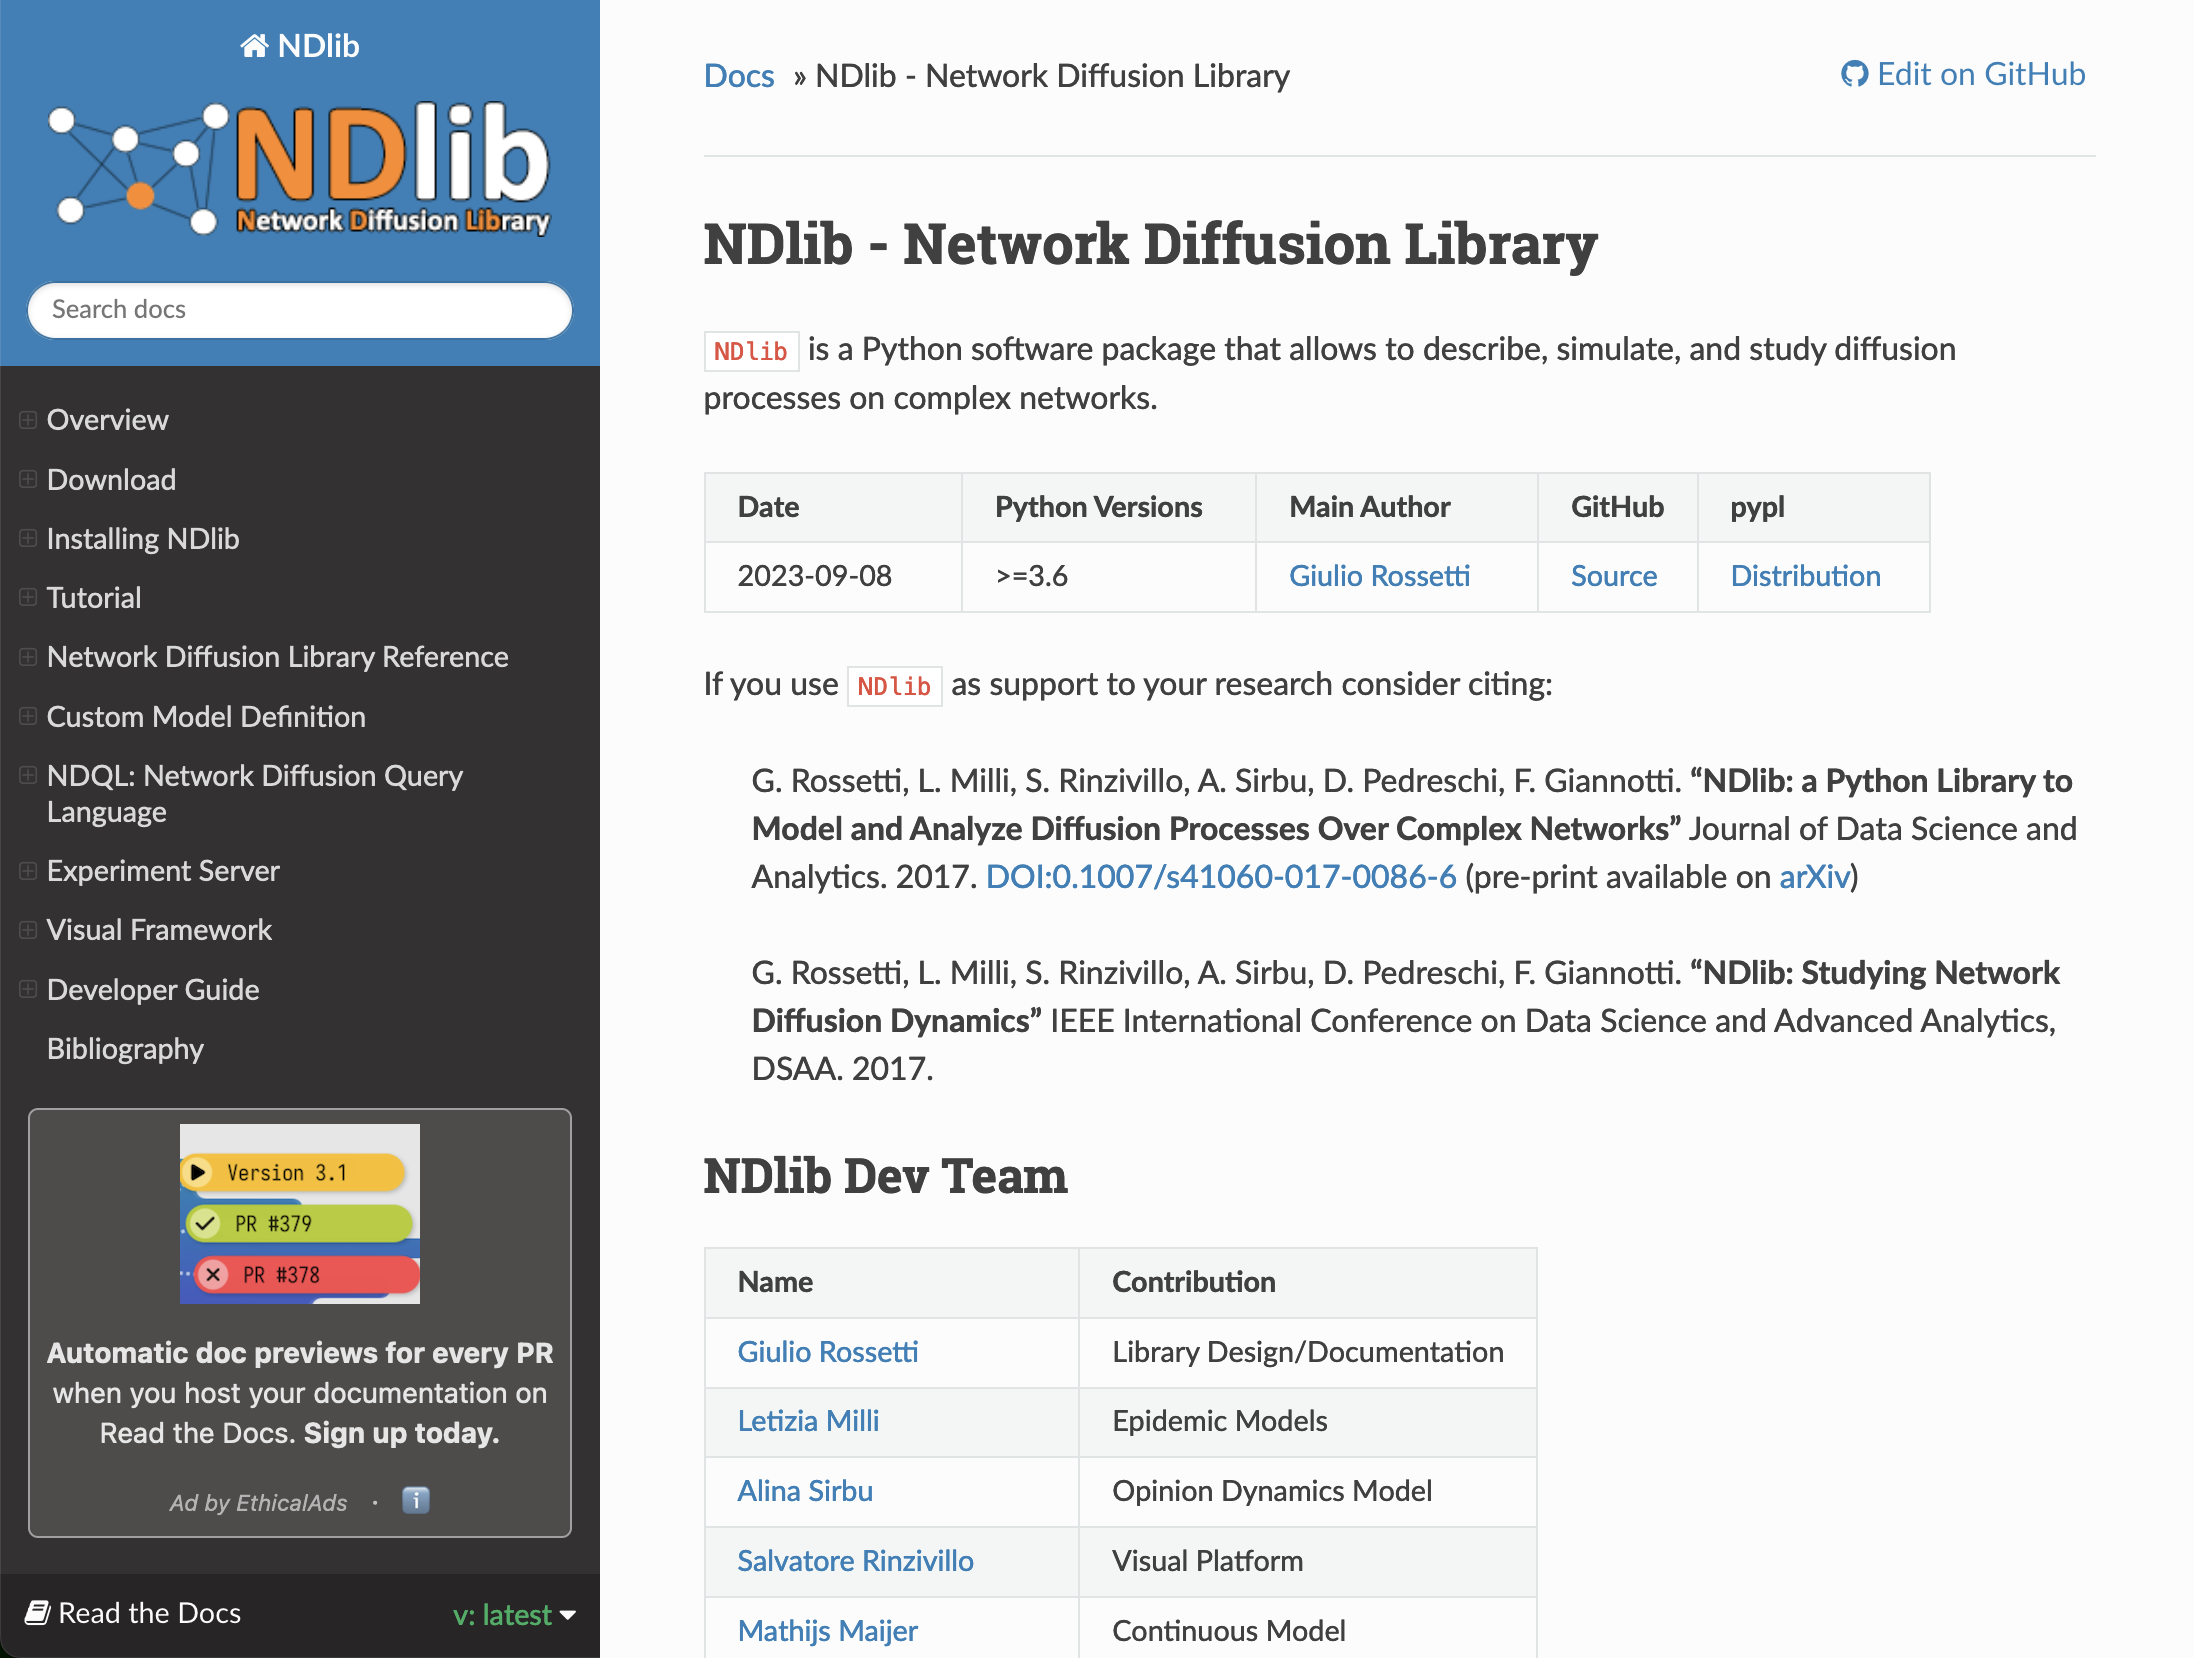
\includegraphics[width=1\textwidth]{figures/ndlib.png}
                \caption{NDlib's website.}
            \end{figure}
        \end{column}
    \end{columns}
\end{frame}

\begin{frame}{\secname}
    However, if we consider...\\
    \vspace{1em}
    \hspace{3em}...more complex network models,... \\
    \vspace{1em}
    \hspace{3em}...spreading multiple processes at the same time... \\
    \vspace{1em}
    \hspace{10em}...\textbf{a gap among the available toolkits} emerges.
\end{frame}

\begin{frame}{\secname}
    \onslide<1->{A focus of our research group is oriented i.a. to: multilayer networks,
    temporal networks, spreading phenomena, data streams.}
    \onslide<2->{\begin{center}
        \arrowdown
    \end{center}
    As a result of our recent activities, we decided to merge and wrap up a code we developed
    into a reusable library. We also decided to to share it with the community in an attempt of
    filling the gap in.}
    \onslide<3->{\begin{center}
        \arrowdown
    \end{center}
    The main operating principles that we determined were:
    \begin{enumerate}
        \item compatibility with other tools commonly used in data science,
        \item development of a tool as a framework with open interfaces,
        \item supporting both multilayer and temporal networks,
        \item supporting spreading models with discrete states.
    \end{enumerate}}
\end{frame}

\section{Key Features}

\begin{frame}{\secname}
    Functionalities of \lstinline[style=py]{network-diffusion}:
    \vspace{1em}
    \begin{itemize}
        \item end-to-end simulation workflow,
        \item predefined spreading models (for multilayer and temporal networks),
        \item an interface for implementing custom spreading models,
        \item support for the temporal network models (CogSNet + discrete windows),
        \item support for the multilayer networks,
        \item centrality measures for multilayer networks.
    \end{itemize}
\end{frame}

\begin{frame}{\secname}
    Environmental requirements for \lstinline[style=py]{network-diffusion}:
    \vspace{1em}
    \begin{itemize}
        \item support for Linux, macOS, and Windows\footnote{Although we develop and use it mostly on Unix OSs},
        \item Python (preferred 3.10) compatibility,
        \item C snippets in the CogSNet module to speed-up computations,
        \item NetworkX compatibility.
    \end{itemize}
\end{frame}

\begin{frame}[fragile]{\secname}
    To prepare the experiment we have to provide a network, a spreading model and auxiliary parameters.
    Then, the simulation unfolds as follows:
    \begin{algorithmic}[1]
        \Procedure{\lstinline[style=py]{perform_propagation}}{\lstinline[style=py]{network, model, epochs*}}
        \State \lstinline[style=py]{states_0} $\gets$ \lstinline[style=py]{model.determine_initial_states()}
        \State \lstinline[style=py]{model.update_network(states_0)} % \Comment{Predefined function in the \texttt{BaseModel} class}
        \For{\lstinline[style=py]{e} in \lstinline[style=py]{[1, ..., epochs]}}
        \State \quad \quad \lstinline[style=py]{states_e} $\gets$ \lstinline[style=py]{model.network_evaluation_step(network)}
        \State \quad \quad \lstinline[style=py]{model.update_network(network, states_e)}
        \EndFor
        \State \lstinline[style=py]{logs} $\gets$ generate logs from experiment \\
        \Return \lstinline[style=py]{logs}
        \EndProcedure
    \end{algorithmic}
\end{frame}

\section{Example I - a Predefined Model}

\begin{frame}{\secname}
    In this example, we will see how to trigger spread under the Linear Threshold Model within a 
    simple, multilayer network.
    \begin{block}{Linear Threshold Model}
    Each node:
    \begin{itemize}
        \item can fall in two states: \textit{active} and \textit{inactive},
        \item becomes \textit{active} if the fraction of its \textit{active} neighbors to all neighbours
        exceeds certain threshold.
    \end{itemize}
    \end{block}
    In case of multilayer networks the actors not the nodes\footnote{which can be considered as avatars
    of the actors on the network's layers} are a subject of the diffusion. Thus, we have to define
    how to aggregate impulses from the layers. In this example we will consider "OR" strategy, which 
    says that the actor can be activated if any of nodes representing it in the network gets activated.
\end{frame}

\begin{frame}{\secname}
    \begin{figure}
        \centering
        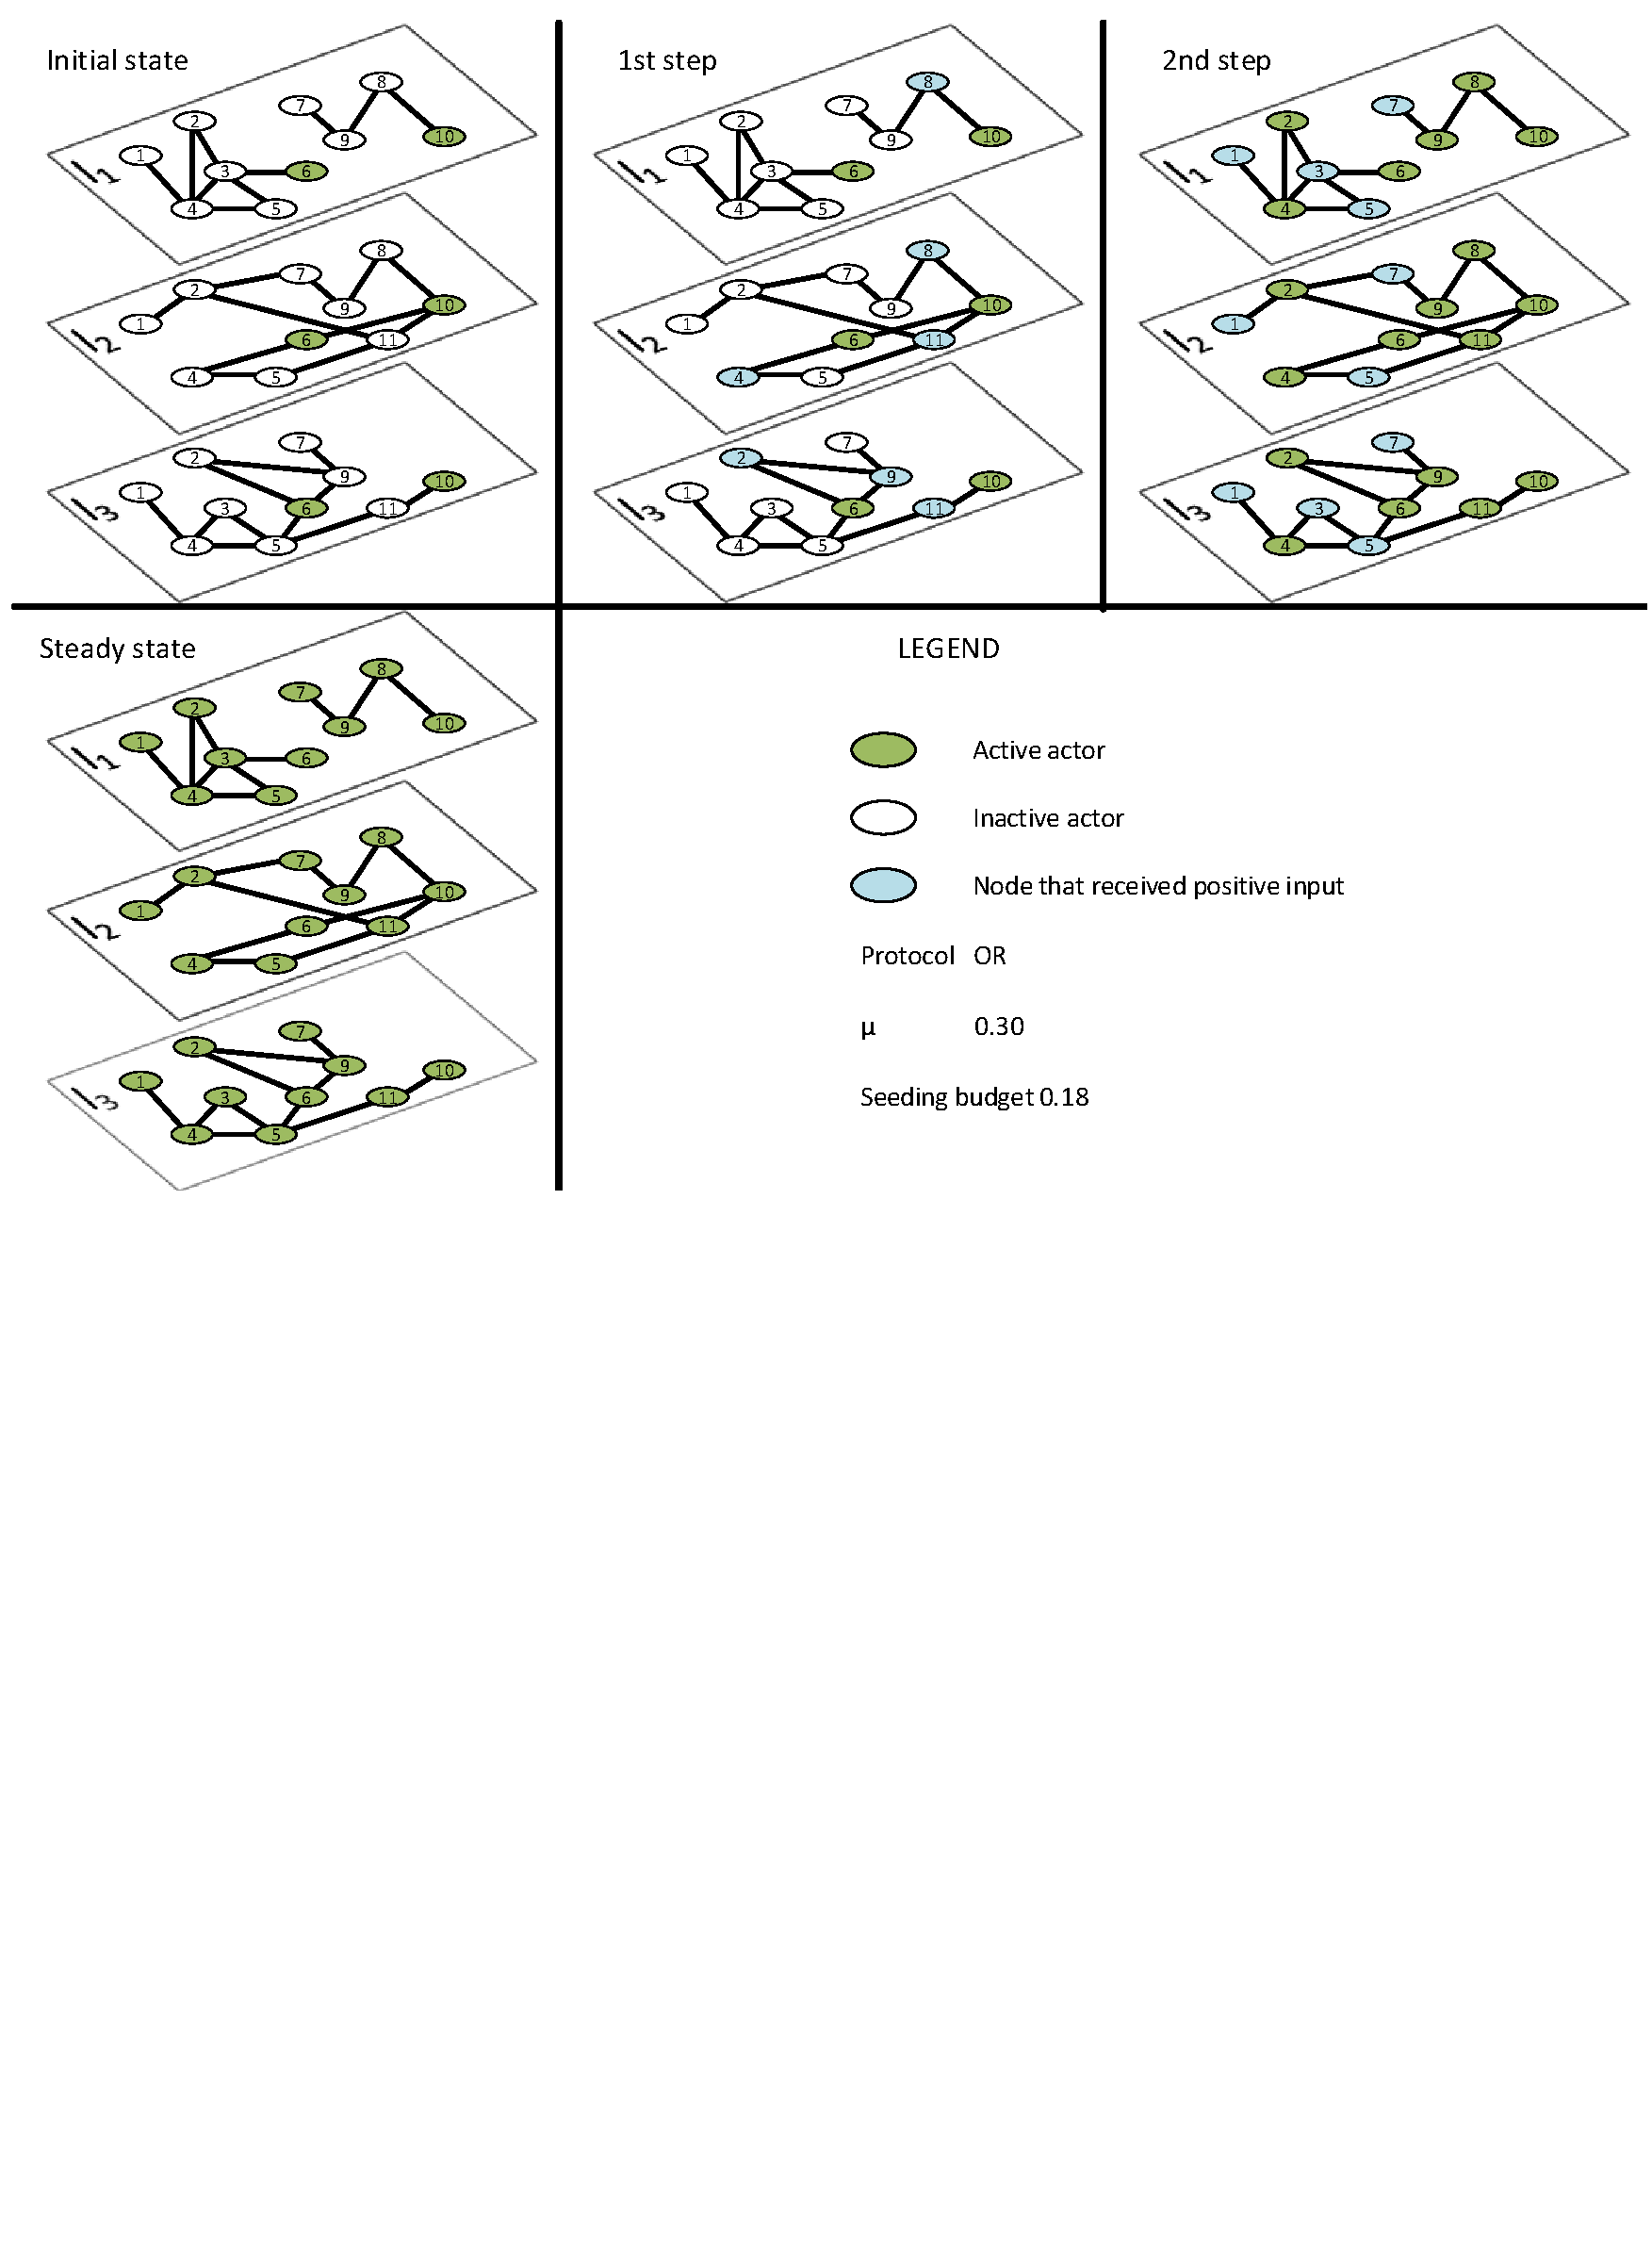
\includegraphics[width=.75\textwidth]{figures/ltm_example_or.pdf}
        \caption{Propagation according to LTM with the $OR$ strategy in a multilayer network -
        active actors: seeds $\{6, 10\}$, in a stable state: all of them.}
    \end{figure}
\end{frame}

\begin{frame}{\secname}
    \begin{center}
        \large Let's model this problem with \lstinline[style=py]{network-diffusion}!
    \end{center}
\end{frame}

\section{Example II - a Custom Model}

\begin{frame}{\secname}
    In this example we will consider a joint disease-awareness model (SIR-UA) that can be used e.g.
    to assess the effectiveness of various countermeasures against the spread of COVID-19 
    (\textbf{see the next presentation for details}):
    \begin{columns}[T]
        \captionsetup{font=scriptsize}
        \begin{column}{.5\textwidth}
            \begin{table}
            \centering
            \caption{Transition weights with explanation.}
            \resizebox{.7\textwidth}{!}{%
            \begin{tabular}{c|p{4cm}}
            Symbol & Description \\ \hline
            $\alpha$ & probability of infection for unaware agents \\ \hline
            $\alpha'$ & probability of infection for aware agents \\ \hline
            $\beta$ & probability of recovery \\ \hline
            $\gamma$ & probability of awareness for uninfected agents \\ \hline
            $\delta$& probability of awareness for infected agents \\
            \end{tabular}%
            }
            \end{table}
        \end{column}
        \begin{column}{0.5\textwidth}
        \begin{figure}
            \centering
            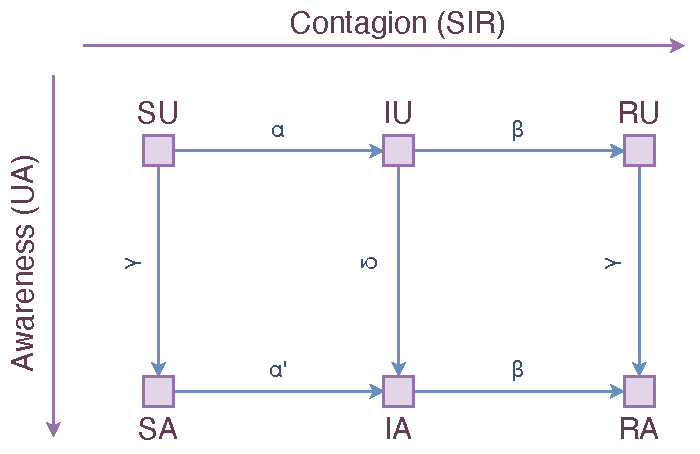
\includegraphics[width=\textwidth]{figures/sir_ua.pdf}
            \caption{State and transition graph for SIR-UA.}
        \end{figure}
        \end{column}
      \end{columns}
\end{frame}

\begin{frame}{\secname}
    To create an own spreading model, we have to extend the abstract base class
    (\lstinline[style=py]{nd.models.BaseModel}) by implementing:
    \begin{itemize}
        \item a field \lstinline[style=py]{_compartmental_graph},
        \item a field \lstinline[style=py]{_seed_selector},
        \item a method \lstinline[style=py]{determine_initial_states},
        \item a method \lstinline[style=py]{agent_evaluation_step},
        \item a method \lstinline[style=py]{network_evaluation_step},
        \item methods \lstinline[style=py]{__str__} and \lstinline[style=py]{get_allowed_states}.
    \end{itemize}
    \vspace{1em}
    The following entities (with implemented method \lstinline[style=py]{update_network}) are
    utilised in the class \lstinline[style=py]{nd.Simulator} which orchestrates the experiment.
\end{frame}

\begin{frame}{\secname}
    \begin{center}
        \large Let's model this problem with \lstinline[style=py]{network-diffusion}!
    \end{center}
\end{frame}

\section{Resources and References}

\begin{frame}[fragile]{\secname}
    The library can be installed via:
    \begin{center}
        \large
        \begin{verbatim}
            pip install network-diffusion
        \end{verbatim}
    \end{center}
    Other useful resources have been also published:
    \begin{itemize}
        \item PyPI website: \url{pypi.org/project/network-diffusion}
        \item GitHub page: \url{github.com/anty-filidor/network_diffusion}
        \item Reference guide: \url{network-diffusion.readthedocs.io}
        \item A preprint of the paper: \url{arxiv.org/abs/2405.18085}
    \end{itemize}
\end{frame}

\section{Limitations of \lstinline[style=py]{network-diffusion}}

\begin{frame}{\secname}
    There is still some work to do...
    \begin{itemize}
        \item implemented in Python ---  performance can be better (only CogSNet implemented in C),
        \item limited to discrete spreading models,
        \item much less pre-defined spreading models than in NDlib,
        \item no user interface --- a limitation for non-programmers,
        \item GPL licence.
    \end{itemize}
\end{frame}

\begin{frame}[allowframebreaks]
    \frametitle{References}
    \bibliographystyle{amsalpha}
    \bibliography{references.bib}
\end{frame}

\addtocounter{framenumber}{1}

\end{document}
